\hypertarget{group__mainpage}{\section{intro\-Hardware Introduction To The Hardware}
\label{group__mainpage}\index{intro\-Hardware Introduction To The Hardware@{intro\-Hardware Introduction To The Hardware}}
}
  
\begin{DoxyImageNoCaption}
  \mbox{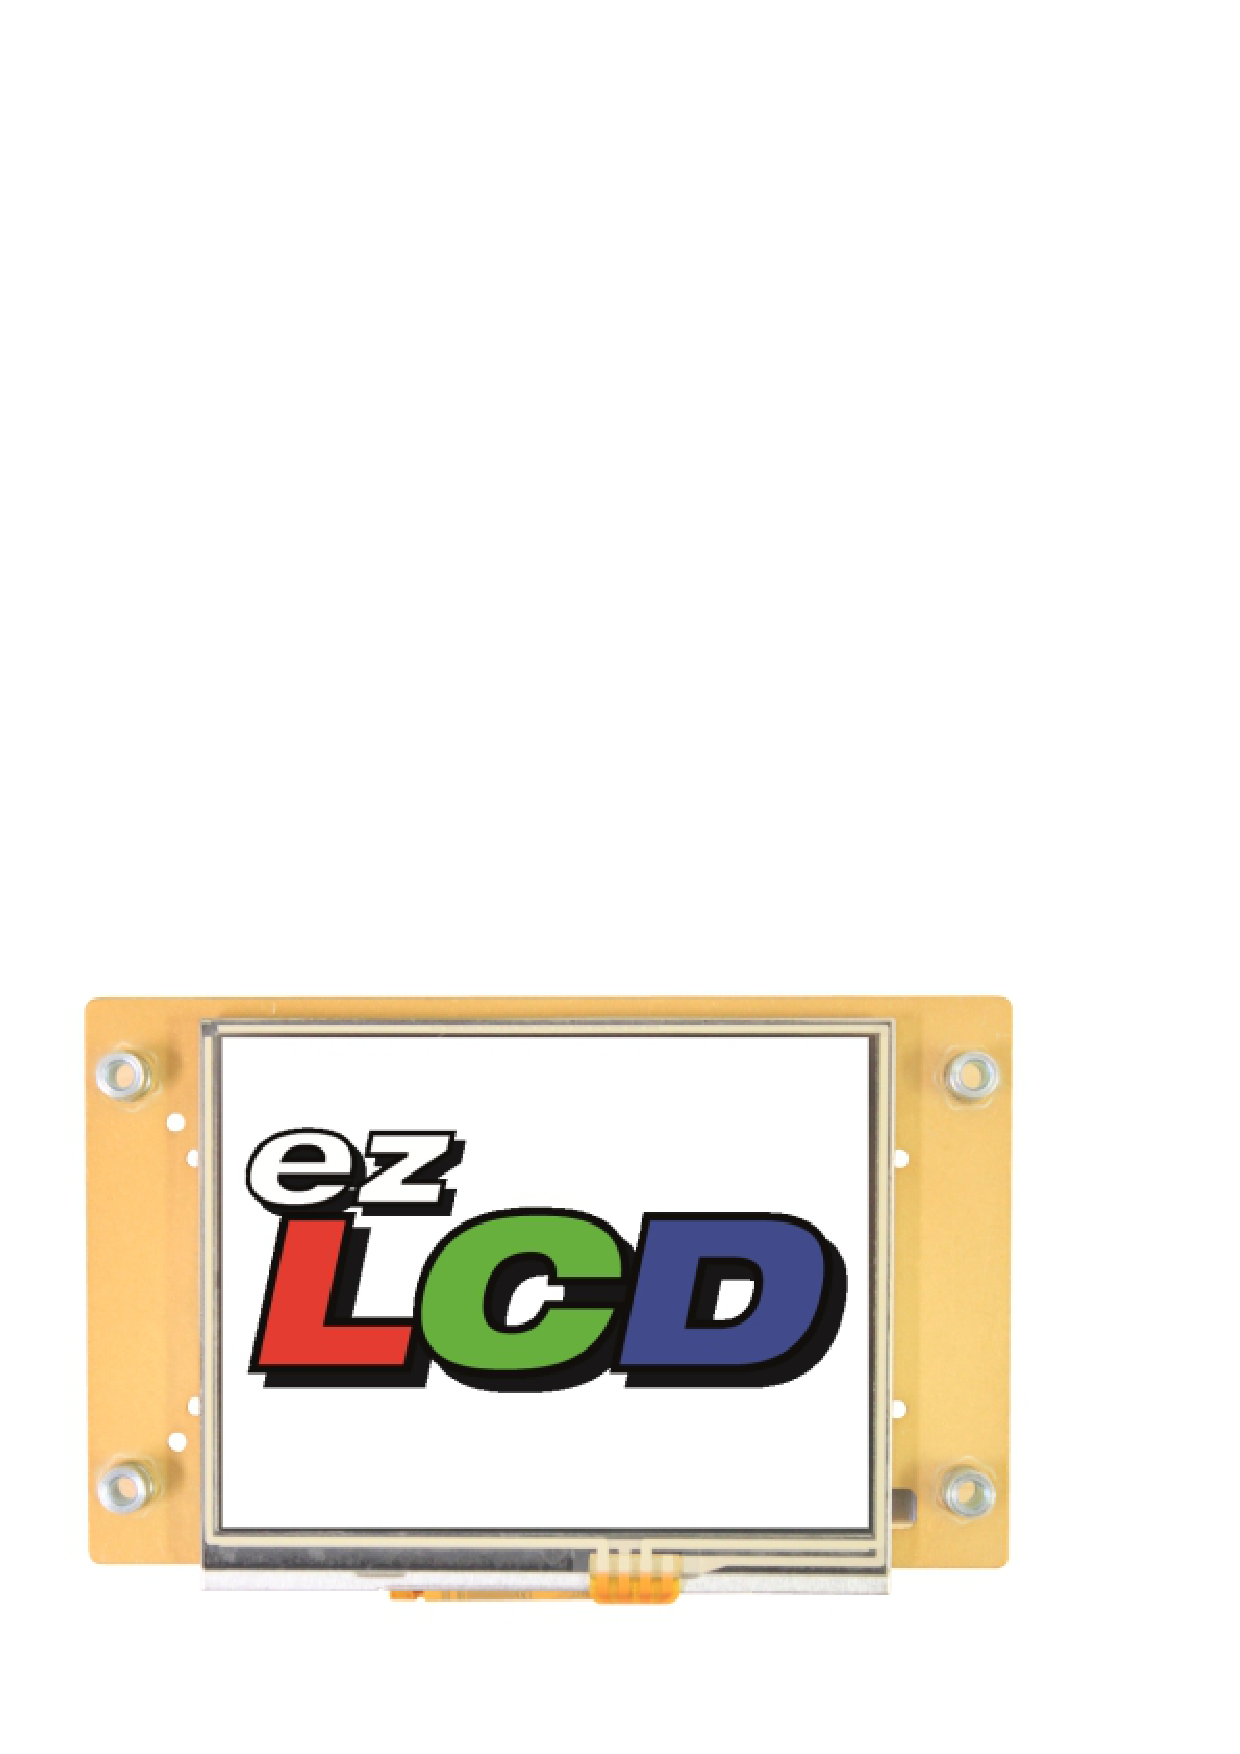
\includegraphics{ezLCD-303Front.png}}
\end{DoxyImageNoCaption}
 
\begin{DoxyImageNoCaption}
  \mbox{
\includegraphics{python.png}}
\end{DoxyImageNoCaption}


The way the \hyperlink{classez_l_c_d3xx_1_1ez_l_c_d}{ez\-L\-C\-D} works \-:\par
 Commands are sent to the \hyperlink{classez_l_c_d3xx_1_1ez_l_c_d}{ez\-L\-C\-D} though the serial interface, Commands are text based and end with a carrage return {\bfseries cr}.\par
 So if you send {\bfseries cls} ending with a {\bfseries cr} the device will clear the screen and return a {\bfseries cr} when the command is complete,\par
 some widgets take a bit of time to complete so after sending a command allways wait for a {\bfseries cr} to comeback before sending another command.\par
 